\chapter[Mixture Models and Model Selection]{Mixture Models and Model Selection}
\markboth{Mixture Models and Model Selection}{}
\label{ch:mixmodels}

\begin{fquote}[Samuel Karlin]The purpose of models is not to fit the data but to 
sharpen the questions.\fqsource{$11^{th}$ R A Fisher Memorial Lecture (1983)} 
\end{fquote} 

\begin{synopsis}
This chapter introduces mathematical foundation and 
formulation of mixture models. The chapter also discusses the
model selection in mixture models.
This chapter also discusses one of the associated publications
where we propose a computationally efficient algorithm to train
a series of mixture models to aid model selection procedure.
\end{synopsis}

Classical probability distributions such as Gaussian, Bernoulli, and 
Poison provide methods for probabilistic modelling 
of data~\cite{walpole2012}. However, in the real world scenario, 
a single probability distribution cannot emulate the complexity 
in the data. Nevertheless, a combination of sufficiently large number 
of probability distributions can possibly emulate complexity in the data. 
Such combination of multiple classical probability distributions 
forms a mixture model. Formally, mixture models are semiparametric 
latent variable models that model a complex data distribution by
weighted sum of different probability 
distributions~\cite{bishop06,everittmixdist,mclachlanfmm}. 

The probability distributions within a mixture model, known as 
component distributions, describe the observations present in the 
data. The formulation of mixture model involves determining the 
number of components in the mixture model, their associated 
distribution, and identification of the component
generating the specific data sample~\cite{mclachlanfmm}. 
Mixture models are often used  in hard clustering analysis as in 
this thesis. In hard clustering, only one component is responsible 
to generate a  specific data sample. Mixture models also provide 
the option of learning soft clustering.  In soft clustering, 
a data sample belongs to more than 
one cluster with a certain degree of association~\cite{bishop06}. 
A standard formulation of the mixture model assumes that the samples 
are independent and identically distributed (IID). Under the assumption 
that data originates from a known number of components, $J$, the 
probability density of a mixture model can be expressed as the weighted
sum of its component distributions as:

\begin{eqnarray}
\label{eq:mixmodel}
 p(x)=\displaystyle\sum_{j=1}^{\mathrm{J}} \pi_j P_j(x \mid \boldsymbol{\theta}_j),
\end{eqnarray}

where $j$ indexes the component distributions. In the 
Equation~(\ref{eq:mixmodel}), the mixing proportion 
(mixing or mixture coefficient) is denoted by $\pi_j$ for the $j^{th}$
component in the mixture model. It determines the weight of the 
component distribution in the overall mixture model. 
Mixing proportions satisfy  the property of convex combination such that 
$\int p(x)dx=1$, $\pi_j > 0$, and $\sum_{j=1}^{J}\pi_{j}=1$~\cite{everittmixdist}. 
Similarly, the parameters $\boldsymbol{\theta}_j$ in  
Equation~(\ref{eq:mixmodel}) denotes  the parameters 
of the $j^{th}$ component distribution of the mixture model.
Application area dictates the choice of distributions, which 
in literature is dominated by the distributions from exponential 
family such as Gaussian, and  Dirichlet~\cite{mclachlanfmm}. 
In this thesis, Bernoulli distribution is the preferred distribution 
because the datasets are 0--1 datasets describing chromosomal
amplifications.

\section{Mixture Models of 0--1 Data}
\label{s:mixmdl01}
Finite mixture model of multivariate Bernoulli distributions 
for a data\-set, $\boldsymbol{X}$, of
dimensionality, $d$, are parametrized by 
$\boldsymbol{\Theta}=\{J$, $\{ \pi_j,\Theta _j\}_{j=1}^{J}\}$. 
The data\-set, $\boldsymbol{X}$, consists of samples
$\mathbf{x}_1, \ldots, \mathbf{x}_N $ in such a way that
$\boldsymbol{X} = \{\mathbf{x}_1, \ldots, \mathbf{x}_N \}$.
Replacing the general probability distribution function with 
the distribution of choice, i.e., Bernoulli distribution, 
a mixture model of multivariate Bernoulli distribution can 
be mathematically expressed as~\cite{everittmixdist,wolfe70}:

\begin{eqnarray}
\label{eq:mixmdl01data}
p(\mathbf{x} \mid \boldsymbol{\Theta})= \displaystyle\sum_{j=1}^{\mathrm{J}} \pi_j \displaystyle \prod _{i=1} ^{\mathrm{d}} \theta_{ji}^{x_i} (1-\theta_{ji})^{1-x_i},
\end{eqnarray}

%As shown in the Equation~\ref{eq:mixmdl01data}, 
 
where $j$ indexes the components,
and $i$ indexes the data dimensionality. $x_i$ denotes the data point 
such that $x_i \in \lbrace 0,1 \rbrace$. The parameter of a random variable $\theta_{ji}$  
denotes the probability of the variable taking the value 1 in $i^{th}$ 
dimension of the $j^{th}$ component. We can collect all the random 
variables in a component in a vector, $\Theta _j$ such that
$\Theta _j=[\theta_{j1},\theta_{j2},\theta_{j3}, \ldots, \theta_{jd}]$.
Similarly, we can collect all the parameters of the mixture model including mixture
components in a matrix, $\boldsymbol{\Theta}$ such
that $\boldsymbol{\Theta}=\{J$, $\{ \pi_j,\Theta_j\}_{j=1}^{J}\}$.
The parameter values that maximise the log--likelihood function 
of the parameters can be defined using 
maximum likelihood principal~\cite{bishop06} as:

\begin{eqnarray}
  \label{eq:loglkhood}
  \mathcal{L} (\boldsymbol{\Theta} \mid \boldsymbol{X}) =\displaystyle\sum_{n=1}^{\mathrm{N}} \log  \left [ \displaystyle\sum_{j=1}^{\mathrm{J}} \pi_j \displaystyle \prod _{i=1} ^{\mathrm{d}} \theta_{ji}^{x_{ni}} (1-\theta_{ji})^{1-x_{ni}} \right].
\end{eqnarray} 
The EM algorithm can be used to learn the maximum likelihood parameters 
of mixture model of Bernoulli  distributions by maximising the likelihood 
in the Equation~(\ref{eq:loglkhood})~\cite{wolfe70}. 

\section{Expectation Maximisation Algorithm}
\label{s:emalgo}
Expectation Maximisation (EM) algorithm is an iterative algorithm
to determine the maximum likelihood (MLE) or maximum a posteriori 
(MAP) estimates of the parameters of latent variable 
models~\cite{expectmax,McLachlan2008emext}. The EM algorithm is a 
popular algorithm for learning model parameters in probabilistic 
latent variable models by maximising the marginal likelihood. 
The iterations of EM algorithm alternate between Expectation 
step (E--Step) and Maximisation Step (M--Step).

E--step estimates the posterior probability of each component 
for every data point. Whereas, M--step updates the  model parameters 
for next iteration. 
Iterations between E and M step produce a succession 
of monotonically increasing sequence of log--likelihood values
for the parameters $\tau\;=\;0,1,2,3,\ldots$ regardless of 
the starting point $\{\pi^{(0)},\Theta^{(0)}\}$~\cite{McLachlan2008emext}. 


\section{Model Selection in Mixture Models }
\label{s:mdlselectmix}

Model selection is the process of selecting a model of optimal complexity 
for the given set of (finite,training) data~\cite{cherkassky1998,hastie09}.
In the statistics literature, model selection is  the process of selecting 
a specific model from a plethora of choices~\cite{kadane04}. For example, 
in classification, model selection may refer to choosing a classification
algorithm from different classification algorithms such as Naive Bayes, 
Decision Trees, and Support Vector Machines. The focus in this thesis is 
modelling of a heterogeneous chromosomal amplification dataset.  
Mixture models are the model of choice because of their ability to model 
heterogeneity and their clustering capabilities. The choice of mixture
models is also motivated by their ability to learn the 
structure of the data better than most other methods because each 
component distributions capture dominant patterns in the data. Furthermore,
mixture models are scientifically proven as learning of mixture models 
involve well studied statistical inference techniques.

In this thesis, model 
selection refers to the model structure selection or complexity 
selection which determines the flexibility of the model to fit or 
explain the data. In other words, model selection in this context 
refers to choosing an appropriate level of model complexity in the 
selected class of model, i.e., mixture model. The complexity parameter 
in mixture  model is the number of component distributions in 
the mixture model. Model selection, therefore, is the selection 
of number of components in the mixture model~\cite{fraley1998}.

EM algorithm requires apriori knowledge of the number of components  
in the mixture model to learn the maximum likelihood parameters from
the data~\cite{McLachlan2008emext}. However, the number of component
distributions are often unknown apriori. Furthermore, one of the major
objectives of machine learning and data mining challanges in the real 
world can often be restricted to determining the number of components 
in the mixture model. Hence, model selection is essential to learn a 
mixture model using the EM algorithm.

A mixture model with large number of mixture components produces larger 
value for the log--likelihood in Equation~(\ref{eq:loglkhood}). However,
a mixture model with large number of mixture components also overfits 
the data, and generalises poorly on the future unseen data. Additionally, 
mixture models with large number of components increase complexity 
in training of mixture models with respect to both time and  memory.
In contrast, a mixture model with smaller number of mixture components 
underfits the data, and is unable to adequately represent 
the underlying data structure. Therefore, model selection aims to 
optimise this tradeoff between too simple and complex models.


\subsection*{Related work in Model Selection in Mixture Models}
\label{ss:relatedmxmdl}

A plethora of criteria and methods have been proposed in the literature
to determine the optimal number of mixture components in a mixture 
model~\cite{mclachlanfmm}. For example, authors 
in~\cite{celeux07},~\cite{Figueiredo2002}, and~\cite{oliveira05} 
provide comprehensive 
review of deterministic, stochastic and resampling criteria
for model selection. Deterministic criteria consists of 
Akaike Information Criterion (AIC)~\cite{akaike1973}, Bayesian 
Information Criterion (BIC)~\cite{schwarz78}, Minimum Description
Length (MDL)~\cite{rissanen1978}, and integrated classification 
likelihood (ICL)~\cite{biernacki2000}. Similarly,  stochastic 
methods includes Markov Chain Monte Carlo (MCMC)~\cite{bensmail97},
and resampling methods includes bootstrapped likelihood ratio 
test~\cite{McLachlan1987}. Similarly, authors in~\cite{woo2006}
propose a robust approach against model misspecification leading 
to a better fitting mixture density based on minimum Hellinger 
distances. In addition, the authors in~\cite{chen2008} 
and~\cite{huang2013model} use penalised likelihood method 
for model selection in mixture model.

Data likelihood is often used as 
the measure of the quality of mixture models~\cite{mixmodelcv}.
A well trained mixture model with appropriate number of mixture
components estimates the underlying data distribution better and 
produces high likelihood values for the unseen data. In addition, 
cross--validation have been popular model validation technique
in the literature~\cite{geisser1974,monsteller1968,stone1974}.
Hence, in this thesis we use cross--validated log--likelihood as 
a criteria for model  selection.


\section{Fast Progressive Training of Mixture Models}
\label{s:fast}

The EM algorithm is sensitive to initialisation and susceptible 
to local optima~\cite{McLachlan2008emext,wu1983}. One solution
to avoid local optima is to run the EM algorithm from different 
random initialisations and select the model with highest likelihood 
as the global optimum. Similarly, another solution is to take the 
average of different runs as general performance of the 
model~\cite{tikka2007b}. Furthermore, the  EM algorithm is 
computationally expensive because of its slow monotonic convergence 
property~\cite{McLachlan2008emext}. Therefore, multiple restart 
strategy is popular method in literature where the EM algorithm 
is run only for a small number of steps, i.e., not until 
convergence, generating large number of models. Among those models, 
the model with maximum likelihood can be selected
to continue training until  convergence~\cite{chickering1997}. 


Similarly, different sophisticated algorithms have been proposed to alleviate
the problem of local optima in EM algorithm, for example, using splitting and 
merging of mixture components~\cite{karciauskas2007,ueda2000}. In~\citepub{j1}, 
we use merging of mixture components as in~\cite{ueda2000} to train a series 
of mixture models. The aim is to aid the model selection algorithm to select 
a model of appropriate complexity, not to avoid local optima. We train multiple 
models with highest number of component distributions and select the best models
among them to start the chain of mixture models by merging the similar mixture
components. The training strategy to generate the chain of mixture models 
resembles  backward elimination methodology in feature 
selection literature~\cite{guyon2003}. We initially start 
with large number of mixture components and progressively 
merge the similar components until the number of components is 1.
We use an approximation of Kullback 
Leibler (KL) divergence as a measure of similarity between 
the two components in the mixture model.

\subsection{Kullback Leibler Divergence and Approximation}
\label{ss:approxKL}

Kullback Leibler (KL) divergence is a nonsymmetric measure of difference 
between two probability distributions~\cite{kullbackleibler51kl}. 
%Given two probability distributions $P$ and $Q$ on a finite set 
%$\boldsymbol{X}$,
The KL divergence between two given probability distributions $P$ and $Q$ 
on a finite set $\boldsymbol{X}$ is symmetrized by adding the KL divergence 
from $P$ to $Q$ and $Q$ to $P$~\cite{juang85}. 

\begin{eqnarray}
  \label{eq:symmc}
  \mathcal{D}_{KL}(P||Q)+\mathcal{D}_{KL}(Q||P) & =  &\displaystyle\sum_{i} P(i) log  \frac{P(i)}{Q(i)}+\displaystyle\sum_{i} Q(i) log \frac{Q(i)}{P(i)}  \nonumber \\
  & = &\displaystyle\sum_{i} \left[ \{ P(i)-Q(i) \} log \frac{P(i)}{Q(i)}\right],
\end{eqnarray}

where $i$ indexes all possible combinations of data elements.
Extending the KL divergence in Equation~(\ref{eq:symmc}), the KL divergence between 
two components of a mixture model for data of dimension, $d$, indexed by $k$ 
for two component distributions $\theta$ and $\beta$ have been derived 
in~\cite{adhikari12ds} as:

\begin{eqnarray}
\label{eq:final2sum} 
KL_{\theta\beta} & = & \displaystyle \sum_{i=1}^{2^{{d}}} \left[ \left\{ \displaystyle \prod _{k=1}^{{d}}  \left(\theta_k^{x_{ik}}(1-\theta_{k})^{(1-x_{ik})} \right)  -\displaystyle \prod _{k=1}^{{d}} \left(  \beta_{k}^{x_{ik}}(1-\beta_{k})^{(1-x_{ik})} \right) \right\} \nonumber \right. \\ 
& & \left. \boldsymbol{\cdot} \; \displaystyle \sum_{k=1}^{{d}} \; log \; \frac{\theta_{k}^{x_{ik}} (1-\theta_{k})^{(1-x_{ik})}} { \beta_{k}^{x_{ik}}(1-\beta_{k})^{(1-x_{ik})}} \right],
\end{eqnarray}

where $x_{ik}$ denotes an element in
$k$th dimensionality of $i$th sample in the data matrix. The 
Equation~(\ref{eq:final2sum}) is the sum of a large number of elements. 
If the dimensionality of the data is 5 then we iterate 32 times and  
when the dimensionality is 20, we iterate more than a million times 
(1,048,576). Moreover, the number of comparisons in a mixture model
having $J$ components for data of dimensionality $d$ is $2^{d}J^{2}$ 
which is computationally expensive. Therefore, in~\citepub{j1}, we 
derive a computationally efficient approximation of the  KL divergence as:

\begin{eqnarray} 
\label{eq:symmcf}
KL_{\theta\beta}  =  \displaystyle \sum_{i \in x^{*} } \left\{ \displaystyle \prod _{k=1}^{{d}}  \left(\theta_k^{x^{*}_{ik}}(1-\theta_{k})^{(1-x^{*}_{ik})} \right) -\displaystyle \prod _{k=1}^{{d}} \left(  \beta_{k}^{x^{*}_{ik}}(1-\beta_{k})^{(1-x_{ik})} \right) \right\},
\end{eqnarray}

where 
$X^{*}=\{x^{*}:x^{*}\in \overline{\underline{\boldsymbol{X}}}\}$ 
is a set of all the unique data samples present in  the dataset
denoted by $\overline{\underline{\boldsymbol{X}}}$. 
Here, the summation is approximated only with  
the samples present in the data.  Similarly, we remove  the fraction 
containing the log term from Equation~(\ref{eq:final2sum}). 
In~\citepub{j1}, we are primarily interested 
in determining  the two closest component distributions in a mixture 
model. We are not necessarily interested in the exact minimum values
of  KL divergence between two component distributions in a mixture  
model. These approximations can inaccurately identify two 
components  as most similar to each other while they differ 
considerably in the full and accurate KL divergence.  

The inaccuracies are in the 
form of selection of two dissimilar components in mixture models to
merge.  However, in~\citepub{j1}, we show that our approximation is 
good estimate of the full KL divergence in terms of matching
the two most similar components distributions. Our approximations, 
as reported  in~\citepub{j1}, is considerably more accurate (twenty 
five times) than random matching of the components. Moreover, our 
approximation are  10,000 times faster than full KL
divergence for the data dimensionality twenty. Nevertheless, 
we compensate for any mismatches by retraining the mixture 
models after merging the mixture components. The aim of 
the methodology described in \citepub{j1} is not to propose 
any new model selection criteria but to propose an efficient 
methodology to train a series of mixture models. The models 
in the series are similar to each other except for the number 
of mixture components. 

\subsection{Series of Mixture Models}
\label{ss:series}

In the algorithm proposed in~\citepub{j1}, first, we train a large number of mixture models
with large number of mixture components (20 in our experiments). Second, we then calculate 
the approximated KL divergence among all the pairs of mixture components. The two 
components with minimum approximated KL divergence are then merged as in~\cite{ueda2000}.
The process of merging of mixture components is iterative and continues until the number
of components is 1.
Mathematically, the merging of the mixing proportions of
two candidate component distributions $\pi_{klmin,1}$, and
$\pi_{klmin,2}$ to generate a single component distribution 
$\pi_{merged}$ can be expressed as:
\begin{eqnarray}
\label{eq:mcomp}
\pi_{merged} \; = \; \pi_{klmin,1}\; + \; \pi_{klmin,2}. 
\end{eqnarray}
Merging the mixture components using Equation~(\ref{eq:mcomp})
preserves the properties of mixing proportions such that they 
have to sum to 1. Similarly, we can merge the parameters of 
two candidate mixture components $\Theta_{klmin,1}$ and 
$\Theta_{klmin,2}$ weighted with their mixing components 
to generate parameters for merged component $\Theta_{merged}$ as:

\begin{eqnarray}
\label{eq:wmparam}
\Theta_{merged} \; = \; \frac{\pi_{klmin,1} \; \times \; \Theta_{klmin,1}\; + \; \pi_{klmin,2} \; \times \; \Theta_{klmin,2}} {\pi_{klmin,1} \; + \pi_{klmin,2}}. 
\end{eqnarray}

The parameters of merged component distributions in Equation~(\ref{eq:wmparam})
also satisfy the properties of probability of a random variable, $\theta$ such that
$0 \le \theta \le 1$. The mixture model obtained after merging the mixture
components is retrained before next iteration of merge operation.
This progressive training and merging results in 
a series of mixture models as shown in the Figure~\ref{Fig:series}.

\begin{figure}[h!]
\centering
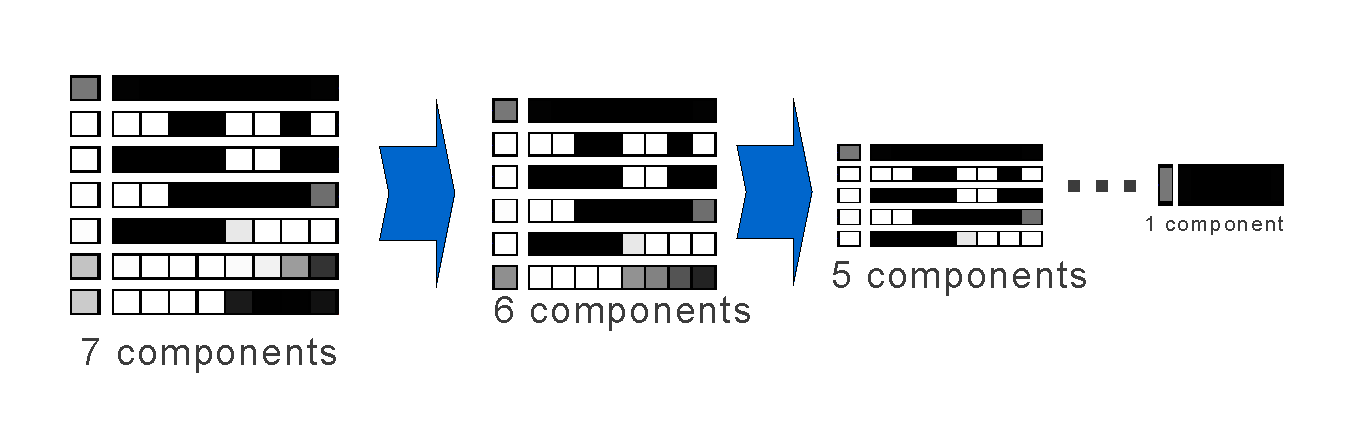
\includegraphics[trim=10mm 10mm 10mm 2mm,width=0.98\textwidth]{figures/seriesofmodels}
\caption[Series of Mixture Models after Merging and Retraining.]
{Series of mixture models resulting from the progressive 
merging of the mixture components and retraining of the mixture 
model. Reprinted with permission from~\citepub{j1}.} 
\label{Fig:series}
\end{figure}

The Figure~\ref{Fig:series} shows snapshot of our algorithm in~\citepub{j1} 
where two components in a mixture model with 7 components are merged 
to generate a mixture model with 6 components. Similarly, mixture 
models with one less components than the previous model are generated 
by merging two most similar component distributions 
until the number of components is 1. The principal focus in~\citepub{j1} is 
generating series of mixture models for model selection 
and not on avoiding local optima or proposing a new 
model selection criteria.

This series of mixture models
can be used with any model selection criteria such as cross--validation,
AIC, BIC, and MDL to choose a model of suitable complexity. In our earlier 
research~\cite{adhikari12ds}, we have used ten--fold cross--validation 
to select model of appropriate complexity. We calculate likelihood of 
each mixture model in the series on both training and validation sets.
We then select the model that generalises the best on the validation
set taking parsimony into account, i.e., if two models produces 
comparable results, we select the simpler model~\cite{zellner2001simplicity}.
In addition to the gain in computational efficiency, the simple models
are also easier to interpret, and understandable to the domain 
experts~\cite{Hollmen2007a}.


One important property of EM algorithm is that EM 
algorithm is deterministic for a given initialisation and
a given dataset~\cite{McLachlan2008emext}. In other words, 
if we run EM algorithm on the same data with same 
initialisation it always converges to the same final model. 
When the mixture components are merged, the initialisation 
for the EM algorithm is same. This avoids multiple 
restarts required in~\cite{chickering1997}~and~\cite{tikka2007b}.
Furthermore, EM algorithm converges faster when it is 
initialised  from a merged model than when initialised 
at random because the merged model resembles the final
trained model. 

In~\citepub{j1}, 
we have shown that EM algorithm converges approximately 
ten to fifty times faster when initialised from  merged 
model. Similarly, the models produced in the series of models
are similar to each other except for the number of 
components. This allows comparison among similar models 
for model selection but with different number of 
components. This avoids the situation when mixture model
with some components have been stuck in local minima while 
models with other components reach global optima. 
Such situations create a bias in comparison among models with 
different components in similar vein as `unfortunate split' in 
cross--validation. 

%The mixing coefficient is denoted by $\pi_j$ for the $j^{th}$
%component in the mixture model. 

% and also 
%of the  model selection in mixture models focusing on the selection of 
%the number of mixture components. 
%Another application area where mixture 
%models have gained prominence is the density estimation.
%~\cite{mclachlanfmm}
%Additionally, mixture models have also been extensively used to 
%handle the missing data for building the model. 
%~\cite{barberBRML12}
%Mixture models have have often been used to combine different density
%models
%~\cite{bishop06}. 
%Mixture models have also been used to model heterogeneity~\cite{mclachlanfmm}. 
%Mixture models have found diverse usage from density estimation 
%to handling missing data~\cite{mclachlanfmm}. However, clustering
%is one of the principal uses of mixture models. 
% 
%A well trained mixture model with appropriate number of mixture component
%models the data generation probabilities and produces high likelihood values
%for the unseen data.








%We capitalize on this property of EM 
%algorithm and merging of mixture components to develop a computationally
%efficient algorithm for model selection.
%Given two probability distributions $P$ and $Q$ on a finite set $\boldsymbol{X}$,
%KL divergence can be mathematically defined as:
%\begin{eqnarray}
%\label{eq:kldiv}
% \mathcal{D}_{KL}(P \mid \mid Q)=\displaystyle\sum_{x \in \boldsymbol{X}} P(x) \log \frac{P(x)}{Q(x)}
%\end{eqnarray}
%However, 
%EM algorithm can get stuck in local optima~\cite{McLachlan2008emext}. 
%The EM algorithm is sensitive to initializations but is deterministic 
%for a given initialization and a given dataset~\cite{McLachlan2008emext}. 
%The symmetric KL divergence satisfies the properties of distance measure such as
%Positivity, Self–similarity, and Self-identification but dissatisfies the 
%triangle equality law~\cite{kullbackleibler51kl}. KL divergence have been
%popular as a difference measure between two probability distribution in
%literature although it is unusable as a metric. 
%The two components selected can mismatch between full
%and accurate KL divergence and our approximation and two inaccurately 
%selected components can be merged.

%We can differentiate Equation~(\ref{eq:loglkhood}) component wise
%with respect to $\theta_{ji}$, and $\pi_{j}$ as:
%\begin{eqnarray}
%\label{eq:em1}
%\frac{\delta \mathcal{L}}{\delta \pi_{j}} = \frac{1}{\pi_{j}} \displaystyle\sum_{n=1}^{\mathrm{N}} P(j|x_n;\pi,\Theta)-N \quad j=1, \ldots, J
%\end{eqnarray}, 
%and
%\begin{eqnarray}
%\label{eq:em2}
%\frac{\delta \mathcal{L}}{\delta \theta_{ji}} = \frac{1}{\theta_{ji}(1-\theta_{ji})} \displaystyle\sum_{n=1}^{\mathrm{N}}P(j|x_n;\pi,\Theta) (x_{ni}-\theta_{ji}), \\
%where \quad j=1, \ldots, J \; and \; i=1,\ldots, d.\nonumber
%\end{eqnarray} 
%The term -N in equation satisfies the constraint $\sum_{j=1}^{J}\pi_j$ introduced in 
%loglikelihood via Lagrange multiplier. The posterior probability can be calculated using 
%Bayes' theorem as:

%\begin{eqnarray}
% \label{eq:emalgo1}
% P(j \mid \boldsymbol{X};\boldsymbol{\Theta})  =  \frac{\pi_j \prod_{i=1}^{d} \theta_{ji}^{x_{ni}}(1-\theta_{ji})^{1-x_{ni}}} {\sum_{j'=1}^{J} \prod_{i=1}^{d} \theta_{j'i}^{x_{ni}}(1-\theta_{j'i})^{1-x_{ni}}}. 
% \end{eqnarray}
 
%We can now define the two step EM algorithm by:

%\textbf{E-step:} In E-step, the posterior probability is computed using 
%Equation~(\ref{eq:emalgo1}) for the most recent values of parameters
%{$\pi ^{\tau}, \Theta ^{\tau}$} at iteration $\tau$, i.e., calculate \\
%$P(j \mid x_n;\pi ^{\tau},\Theta ^{\tau})$.

%\textbf{M-step:} M-step recomputes the values of parameters 
%{$\pi^{(\tau+1)},\boldsymbol{\Theta}^{(\tau+1)}$} for the next iteration as

%\begin{eqnarray}
%\label{eq:mstep1}
%\pi_{j}^{\left(\tau+1\right)} & = & \frac{1}{N} \displaystyle \sum _{n=1}^N P(j \mid x_n;\pi^{(\tau)},\Theta^{(\tau)}), \nonumber \\
%\Theta_{j}^{(\tau+1)} & = & \frac{1}{N \pi_{j}^{(\tau+1)}} \displaystyle \sum _{n=1}^N P(j \mid x_n;\pi^{(\tau)},\Theta^{(\tau)})x_n. 
%\end{eqnarray}